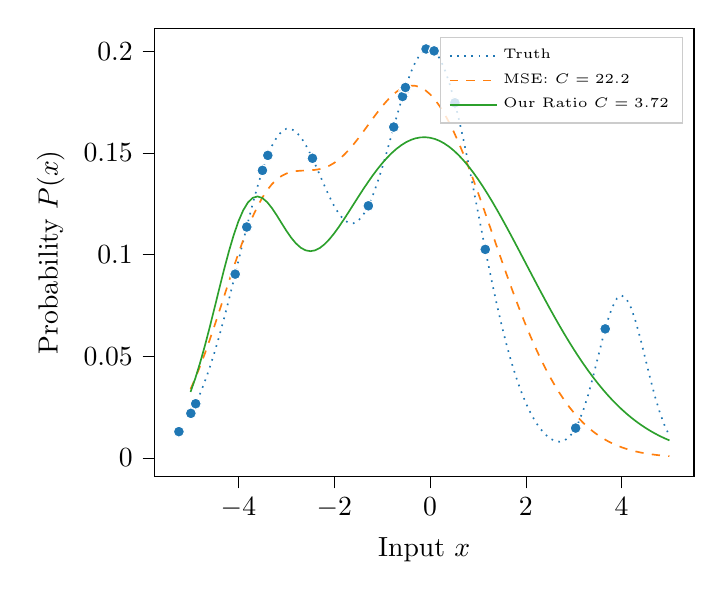
\begin{tikzpicture}

\definecolor{color0}{rgb}{0.12156862745098,0.466666666666667,0.705882352941177}
\definecolor{color1}{rgb}{1,0.498039215686275,0.0549019607843137}
\definecolor{color2}{rgb}{0.172549019607843,0.627450980392157,0.172549019607843}

\begin{axis}[
legend cell align={left},
legend style={fill opacity=0.8, draw opacity=1, text opacity=1, draw=white!80!black},
tick align=outside,
tick pos=left,
x grid style={white!69.0196078431373!black},
xmin=-5.75533199580941, 
xmax=5.51215866646711,
xtick style={color=black},
 legend style={font=\tiny},
y grid style={white!69.0196078431373!black},
ymin=-0.00919013883502155, ymax=0.211264547108374,
ytick style={color=black},
xlabel=Input $x$,
ylabel=Probability $\mathbb{P}(x)$,
yticklabel style={
/pgf/number format/fixed,
/pgf/number format/precision=2
},
]
\addplot [draw=white, fill=color0, forget plot, mark=*, only marks]
table{%
x  y
-2.45408063787313 0.147304544494416
-4.89255956535183 0.0266205286059788
-4.99358897164254 0.0218753976057837
-4.06725898560156 0.090339067875623
-3.82671617251779 0.113517638466833
-3.38654514308717 0.148734482418585
-5.24317332934229 0.0128922881731769
-3.49861669313258 0.14136189107296
-1.28682451616164 0.123940171285403
-0.0826488809022778 0.201054852945502
0.0853628573840893 0.200112947532958
-0.535963859326452 0.18044972528718
1.15419405383195 0.102500353110527
-0.52335572871809 0.181372353460332
-0.572710189621526 0.177686588189846
-0.512970366965474 0.182121828012391
-0.757179225204211 0.162658583433792
0.519640840808635 0.174604611021675
3.65836576443745 0.0634252190990639
3.04092561241004 0.0146345264205772
};
\addplot [semithick, color0, dotted]
table {%
-5 0.0215971299650326
-4.9 0.0262475453902436
-4.8 0.0315820439699032
-4.7 0.0376228158633442
-4.6 0.044373404297815
-4.5 0.0518150301369101
-4.4 0.0599034574899429
-4.3 0.068566704417494
-4.2 0.0777038935271634
-4.1 0.0871855016416088
-4 0.0968552049205398
-3.9 0.106533427695198
-3.8 0.116022594567489
-3.7 0.12511396348198
-3.6 0.133595792121777
-3.5 0.141262472053243
-3.4 0.147924165705566
-3.3 0.153416410653737
-3.2 0.157609121690915
-3.1 0.160414428518905
-3 0.161792836366542
-2.9 0.161757285200693
-2.8 0.160374803381672
-2.7 0.157765593591421
-2.6 0.154099540738172
-2.5 0.149590280952504
-2.4 0.144487106304141
-2.3 0.139065092217505
-2.2 0.133613917527709
-2.1 0.128425897949716
-2 0.123783773064251
-1.9 0.119948778200359
-1.8 0.117149501143732
-1.7 0.115571975507566
-1.6 0.115351403594026
-1.5 0.116565836099303
-1.4 0.119232066689655
-1.3 0.123303926974658
-1.2 0.128673090811964
-1.1 0.135172414426146
-1 0.142581748864847
-0.899999999999999 0.150636063341548
-0.8 0.159035613519234
-0.7 0.167457781780021
-0.6 0.175570113563837
-0.5 0.183043983579577
-0.399999999999999 0.189568257845136
-0.3 0.194862281656031
-0.199999999999999 0.19868752762092
-0.0999999999999996 0.200857286706416
0 0.201243879565493
0.100000000000001 0.199783001360991
0.2 0.196474982268337
0.300000000000001 0.191382935305986
0.4 0.184627957819492
0.5 0.176381736461995
0.600000000000001 0.166857062225207
0.7 0.156296878819335
0.800000000000001 0.144962555252821
0.9 0.133122087496691
1 0.121038895565054
1.1 0.108961797133785
1.2 0.0971166170839501
1.3 0.0856997472498373
1.4 0.0748738170270953
1.5 0.0647654886732916
1.6 0.0554652659403721
1.7 0.0470291147889281
1.8 0.0394816521643415
1.9 0.0328206715851879
2 0.0270228439895529
2.1 0.0220505462727784
2.2 0.0178598912505523
2.3 0.0144100895584638
2.4 0.0116741570821882
2.5 0.00965056300821204
2.6 0.0083745996639208
2.7 0.0079270753097688
2.8 0.00843663975973713
2.9 0.0100711891854397
3 0.0130141199389598
3.1 0.0174234425154325
3.2 0.0233762117541372
3.3 0.0308067779807332
3.4 0.0394533207844047
3.5 0.0488304863581338
3.6 0.0582442615728206
3.7 0.0668573107421607
3.8 0.0738000015380843
3.9 0.0783078665381089
4 0.0798553711968229
4.1 0.0782531696254852
4.2 0.0736834995954261
4.3 0.0666641881771586
4.4 0.0579507817881467
4.5 0.0484021367744795
4.6 0.038842281422721
4.7 0.0299486780397596
4.8 0.0221861475854464
4.9 0.0157912511405562
5 0.010798936662397
};
\addlegendentry{Truth}
\addplot [semithick, color1, dashed]
table {%
-5 0.0337769988002927
-4.9 0.0391890856301241
-4.8 0.0450617060761197
-4.7 0.0513536585627463
-4.6 0.0580075188277943
-4.5 0.0649501189159881
-4.4 0.0720939049502544
-4.3 0.0793391969915272
-4.2 0.0865773125904092
-4.1 0.0936944499084158
-4 0.100576162009936
-3.9 0.107112196990843
-3.8 0.113201434736859
-3.7 0.118756625212261
-3.6 0.123708628792308
-3.5 0.128009877932988
-3.4 0.131636820935071
-3.3 0.134591170024644
-3.2 0.136899852759657
-3.1 0.138613651637296
-3 0.139804604531082
-2.9 0.14056232083128
-2.8 0.140989438049592
-2.7 0.141196495576372
-2.6 0.141296532431264
-2.5 0.141399722533074
-2.4 0.141608344746345
-2.3 0.142012348305034
-2.2 0.142685721407698
-2.1 0.143683807208062
-2 0.145041643000234
-1.9 0.146773330932565
-1.8 0.148872387236503
-1.7 0.151312965797068
-1.6 0.154051813631618
-1.5 0.157030791740462
-1.4 0.160179784718457
-1.3 0.163419825163009
-1.2 0.166666272092131
-1.1 0.169831903573353
-1 0.172829809649127
-0.899999999999999 0.175575999635747
-0.8 0.177991665540352
-0.7 0.18000506877486
-0.6 0.181553039232292
-0.5 0.18258209340963
-0.399999999999999 0.183049191422907
-0.3 0.182922161702327
-0.199999999999999 0.182179827417614
-0.0999999999999996 0.180811870980369
0 0.178818473073886
0.100000000000001 0.176209761310197
0.2 0.173005101447482
0.300000000000001 0.169232261618033
0.4 0.164926477565794
0.5 0.160129444676163
0.600000000000001 0.154888260678486
0.7 0.14925434129798
0.800000000000001 0.143282329750063
0.9 0.137029019695024
1 0.130552309986424
1.1 0.123910208147548
1.2 0.117159897917605
1.3 0.110356884377843
1.4 0.103554228086482
1.5 0.0968018773426022
1.6 0.090146105211665
1.7 0.0836290553485502
1.8 0.077288398029279
1.9 0.0711570952362998
2 0.0652632712186865
2.1 0.0596301827445153
2.2 0.0542762813427077
2.3 0.0492153582455168
2.4 0.0444567615237415
2.5 0.0400056740708529
2.6 0.0358634406392884
2.7 0.0320279320470259
2.8 0.028493934927108
2.9 0.0252535559485199
3 0.0222966302474784
3.1 0.0196111248225479
3.2 0.017183528811539
3.3 0.0149992238295258
3.4 0.0130428288545351
3.5 0.0112985154536449
3.6 0.00975029040605429
3.7 0.00838224396632478
3.8 0.00717876309271695
3.9 0.00612470992188137
4 0.00520556658877074
4.1 0.00440754816285746
4.2 0.00371768599793597
4.3 0.00312388417752937
4.4 0.00261495199004527
4.5 0.00218061549948663
4.6 0.00181151130320267
4.7 0.00149916550377718
4.8 0.0012359607841986
4.9 0.00101509428031263
5 0.000830528707860075
};
\addlegendentry{MSE: $C=22.2$}
\addplot [semithick, color2]
table {%
-5 0.0323958745727326
-4.9 0.0391420064293868
-4.8 0.0467601290230525
-4.7 0.0551605669913342
-4.6 0.0641891745779988
-4.5 0.0736276290264261
-4.4 0.0832006082606963
-4.3 0.0925902014222532
-4.2 0.10145689854078
-4.1 0.109465451244952
-4 0.116312977906749
-3.9 0.121756089981962
-3.8 0.125633683912196
-3.7 0.12788243746355
-3.6 0.128542933442402
-3.5 0.127755571818367
-3.4 0.125746814635934
-3.3 0.122807597450407
-3.2 0.119266716875604
-3.1 0.115462511805566
-3 0.11171613621158
-2.9 0.108309216004522
-2.8 0.105467818929144
-2.7 0.103353624845478
-2.6 0.102062155054464
-2.5 0.10162706659072
-2.4 0.10202894796438
-2.3 0.103206806448911
-2.2 0.105070490118809
-2.1 0.107512570112466
-2 0.110418625796296
-1.9 0.113675332310429
-1.8 0.117176167773461
-1.7 0.120824884448791
-1.6 0.124537101718034
-1.5 0.128240481035566
-1.4 0.131873953648761
-1.3 0.13538641875614
-1.2 0.138735241829921
-1.1 0.141884784548519
-1 0.14480510660951
-0.899999999999999 0.147470905590037
-0.8 0.149860707586822
-0.7 0.151956287677372
-0.6 0.15374228179497
-0.5 0.15520594594447
-0.399999999999999 0.156337020513138
-0.3 0.157127663243832
-0.199999999999999 0.157572421725376
-0.0999999999999996 0.157668223446509
0 0.1574143677351
0.100000000000001 0.156812508964536
0.2 0.155866624269659
0.300000000000001 0.154582961846561
0.4 0.152969967935319
0.5 0.151038192014387
0.600000000000001 0.148800170744627
0.7 0.146270291920867
0.800000000000001 0.143464640210581
0.9 0.140400826842321
1 0.137097805687582
1.1 0.13357567838075
1.2 0.129855491254805
1.3 0.125959026942804
1.4 0.121908593511181
1.5 0.117726813954138
1.6 0.113436418792085
1.7 0.109060044385041
1.8 0.104620039398386
1.9 0.100138281648231
2 0.095636007312504
2.1 0.0911336542274227
2.2 0.0866507207036334
2.3 0.0822056409982603
2.4 0.0778156782747968
2.5 0.0734968355783807
2.6 0.0692637850554585
2.7 0.0651298153596439
2.8 0.0611067969146947
2.9 0.0572051644553313
3 0.0534339160407533
3.1 0.0498006275371427
3.2 0.0463114813963194
3.3 0.042971308419481
3.4 0.0397836410882481
3.5 0.0367507769700113
3.6 0.0338738506601066
3.7 0.031152912708295
3.8 0.0285870139895472
3.9 0.0261742940169027
4 0.0239120717545351
4.1 0.0217969375691552
4.2 0.0198248450544079
4.3 0.0179912015727454
4.4 0.0162909564791677
4.5 0.0147186861180446
4.6 0.01326867481495
4.7 0.0119349912172054
4.8 0.0107115594670551
4.9 0.00959222481775619
5 0.00857081342334995
};
\addlegendentry{Our Ratio $C=3.72$}
\end{axis}

\end{tikzpicture}